% chapter 1
\chapter{Introduction}

This project is about using linear programming (LP) and analysing the different LP tools used to solve vehicle routing problem (VRP).

\section{The Problem}
Furnish ltd\footnote{A fictional company} is a leading furniture store in the UK. It regularly makes door-to-door deliveries to customers
across the country. Making these deliveries cost a lot of money and the company is looking to minimise cost incurred by using delivery routes
that have shorter distances. With this goal in mind, they are hoping to maximise their profits and reduce carbon emissions.

The problem stated above is known as the vehicle routing problem (VRP) \cite{Dantzig1959, Daneshzand2011}. It is a problem where a fleet of vehicles,
which are based on a central location (depot), are required to visit geographically dispersed customers
 to fulfil their respective needs. The main objective is to find the optimal routes for the fleet of vehicles that
 yield the minimum cost, which could be in terms of fuel, time or distance.
VRP has been studied for decades due to its relevance in applied mathematics and wide range of applications in the real world, especially logistics.
Finding optimal routes in logistics industry is a lucrative business, given the fact that the industry is worth approximately \pounds55 billion
in the UK alone\footnote{According to recent report by PWC. Link: \url{http://goo.gl/iDkTe3}}.
Despite being a simple problem to explain, it is notoriously difficult to find an algorithm that can efficiently solve VRP.
It also plays a part towards understanding the P vs NP problem\footnote{
See \url{http://www.claymath.org/millennium-problems/p-vs-np-problem}} by providing a testbed for new algorithms.
A visualisation of VRP is shown in figure 1.1.

\begin{figure}[!ht]
  \centering
    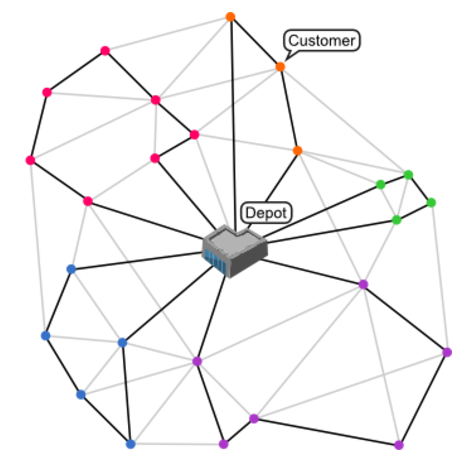
\includegraphics[width=0.6\textwidth]{vrp-sample.png}
    \caption{A visualisation of VRP, taken from Networking and Emerging Optimization \cite{neo:vrp}}
\end{figure}

In this project, we will be using linear programming (LP) to solve VRP. LP is a method to find the optimal allocation
of resources among competing activities in a system of linear equations \cite{APMBradley}. There had been many methods of solving linear equalities
problems since the 19th century, none of which made any significant impact. The turning point came in 1947, where George Dantzig
developed the Simplex method \cite{wiki:SA}, an algorithm to solve LP problems. Simplex method was highly influential
in the development and practice of science and engineering such that it was
listed as one of the top 10 algorithms of the 20th century. It also made a signigicant impact in
 Operations Research (OR), a field of study that concerns with making better decisions through mathematical analysis \cite{wiki:OR}.
 With increasingly higher computational power and
the efficiency of the simplex method, LP has become the most powerful optimisation method that enchance decision making
process.

In this project, we shall act as an OR consultant for the fictional furniture company to solve their vehicle
routing issues and analyse a few popular LP tools, so that they may choose one that is best for their situation.
In addition, we would like to show the readers how to solve optimisation problem using linear programming.

\section{Aims and Goals}
The aims of this project are to find the optimal solutions to an instance of VRP using the LP tools that we have chosen and analyse their features and
performance.
To achieve those aims, we have set up the list of goals below:
\begin{enumerate}
\item To thoroughly understand linear programming and other related concepts to solve problems.
\item To correctly identify the problem and build accurate LP models based on it.
\item To analyse the performance and features of the chosen LP tools.
\item To obtain the optimal solutions: the minimum distance and the vehicle routes, using the chosen LP tool.
\end{enumerate}

\section{Limitations}
Creating novel algorithms for optimisation problems is hard and requires years of experience in algorithms. Furthermore,
implementing linear programming solver is also difficult and it requires very high level of software engineering expertise.
 For these reasons, we will not be attempting to create new algorithms or building new an LP solver to solve
the vehicle routing problem. Instead, we will model the VRP instance using existing softwares and algorithms.
Other methods that are not related to LP, such as genetic programming and dynamic programming will not be discussed in this project.

\section{Methodology}
This project will be carried out in seven steps, adapted from the Sottinen \cite{Sottinen2009}:
\begin{enumerate}
\item Define the problem and formulate it into a linear program. Study the objective and the constraints of the problem thoroughly to ensure
that the linear program accurately represent the given problem.
\item Collect the relevant datasets and their respective parameters.
\item Create the mathematical formulations of the given problem using the standard LP notation.
Then, create the corresponding LP models based on the formulations on all of the LP tools. Each of the chosen LP tools would
have its own LP models based of the same formulations.
\item Verify that the LP models are correct on all tools by running them with a test dataset with known solution. This is a quick test
to determine whether we have modelled the LP models correctly. We may need to go back to step 1 if the results obtained
are not satisfactory.
\item Analyse the performance by testing the LP models
 against the benchmark datasets from Augerat \cite{Augerat1998} and the compare features of the LP tools.
\item Select the best tool to solve the given VRP proble and analyse the given problem using the model implemented in our chosen LP tool.
\item Provide recommendations based on the analysis to the client involved.
\end{enumerate}

\section{Terminologies}
There are a few terminologies mentioned in this project whose meaning are not explicitly stated.
For clarity, we have list down those terminologies along with their respective meaning:
\begin{itemize}
\item Linear/integer Program - An instance of a problem that can be solved using a linear/integer programming method.
\item Formulation - An instance of LP that describes a specific problem.
\item Model (Noun) - An implementation of an LP formulation in an LP tool.
\item Solver - A program that is used to solve LP problems that is based on constraint programming\footnote{refer to chapter 2}.
\item Method - Often used interchangeably with algorithm.
\end{itemize}

\section{Outline of Subsequent Chapters}
We have introduced the reader to this project, describe its goals and how to steps taken to attain them. In chapter 2,
we will provide some contexts for the reader on the theories that we apply in the project. Chapter 3 will focus on
analysing the given problem, including forming the correct LP formulation and identifying the client's requirements.
The implentation of LP formulations using the chosen tools will be discussed in chapter 4, followed by the results and
some their comments in chapter 5. Finally, we will conclude the results and identify potential future works
of this project in chapter 6.